\section{Analyseklasser}
Inden analyseklasserne udarbejdes, foretages en analyse ud fra systembeskrivelsen, use case og funktionaliteter til at identificere substantiver og verber. Dette gøres for at sikre, at alle funktionaliteter indgår i design af klassediagrammer. Substantiver og verber fra analysen fremgår af \autoref{tab:subverb}.

\begin{table}[H]
\centering
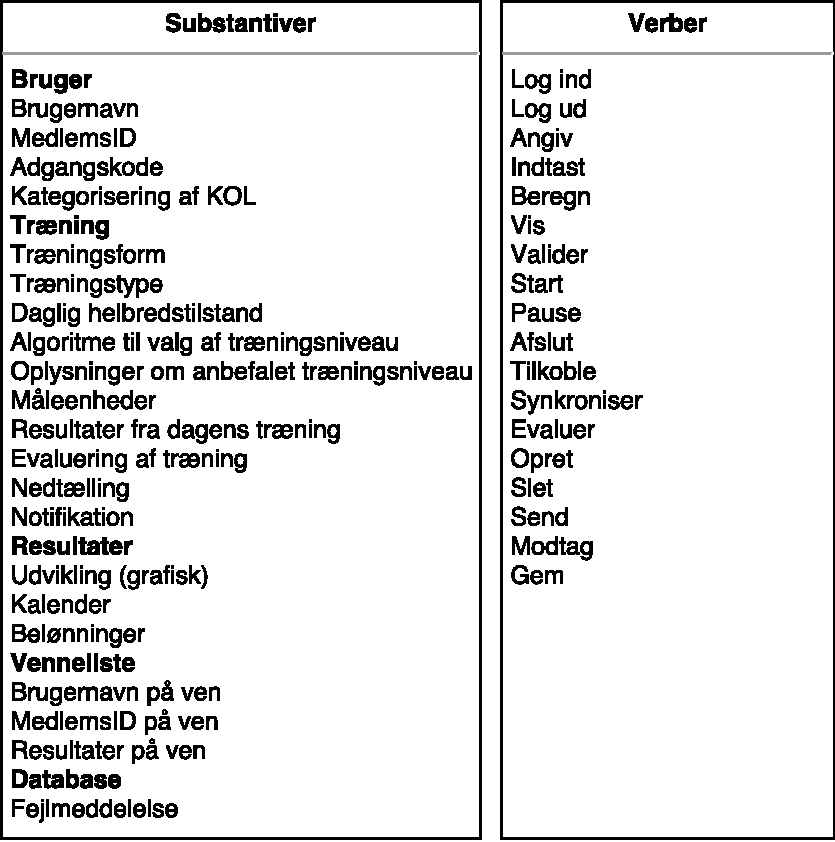
\includegraphics[width=0.7\textwidth]{figures/aktivitetsdiagram/substantiveverber}
\caption{Substantiver og verber identificeret ved analyse af systembeskrivelse, use case samt funktionaliteter.}
\label{tab:subverb}
\end{table}

\noindent
De fremhævede substantiver, brugeroplysninger, træning, resultater, venneliste og database, identificeres som klasser. Under hver klasse fremgår deres tilhørende attributter, der beskriver den overordnede klasse. Verberne betegner de metoder, der kan tilgås i de forskellige klasser. 

Efter substantiver og verber er identificeret inddeles disse i analyseklasser og opdeles i stereotyperne, entity, boundary og control. Dette kan ses af \autoref{fig:analyseklasse}. 

\begin{figure}[H]
\centering
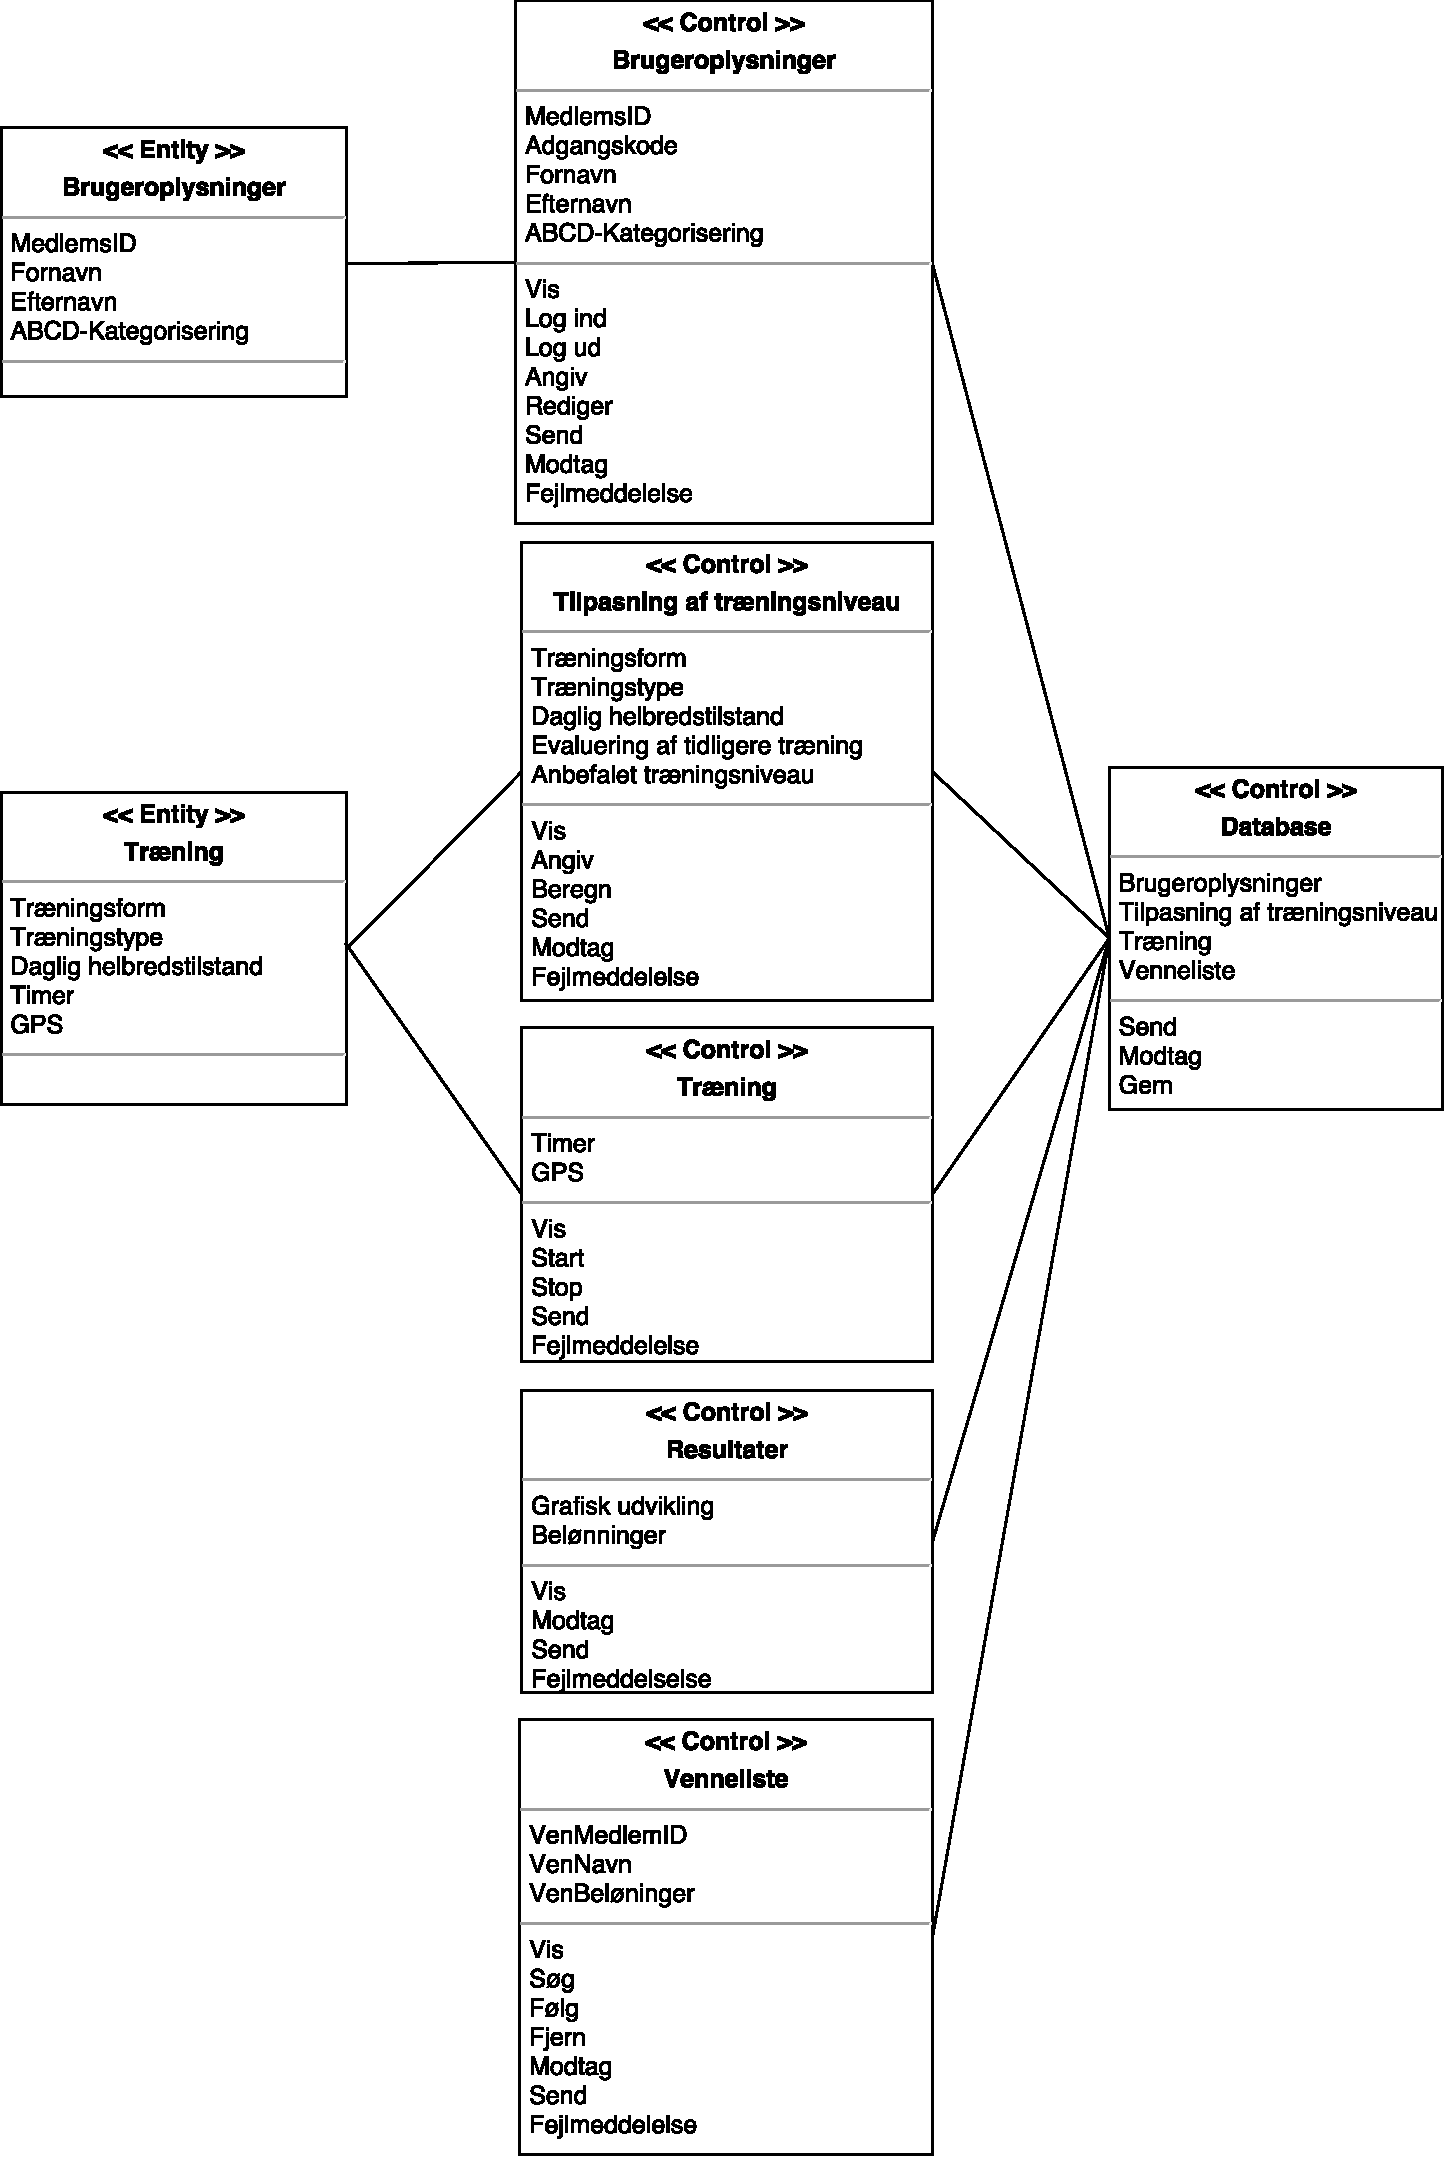
\includegraphics[width=0.7\textwidth]{figures/aktivitetsdiagram/analyseklasser}
\caption{Analyseklasser udarbejdet ud fra de identificerede substantiver og verber.}
\label{fig:analyseklasse}
\end{figure}

\noindent
Af \autoref{fig:analyseklasse} fremgår relationen mellem klasserne og deres tilhørende attributter samt metoder.  \textit{Database} er defineret som entityklasse, da den skal lagre og opdatere informationer. \textit{Resultater} er defineret som boundaryklasse, da den skal vise resultater på en grænseflade.  \textit{Brugeroplysninger}, \textit{Tilpasning af træningsniveau}, \textit{Træning} og \textit{Venneliste} defineres som controlklasser, idet disse anvendes til at kontrollere handlinger. 

